% Options for packages loaded elsewhere
\PassOptionsToPackage{unicode}{hyperref}
\PassOptionsToPackage{hyphens}{url}
%
\documentclass[
]{book}
\usepackage{amsmath,amssymb}
\usepackage{iftex}
\ifPDFTeX
  \usepackage[T1]{fontenc}
  \usepackage[utf8]{inputenc}
  \usepackage{textcomp} % provide euro and other symbols
\else % if luatex or xetex
  \usepackage{unicode-math} % this also loads fontspec
  \defaultfontfeatures{Scale=MatchLowercase}
  \defaultfontfeatures[\rmfamily]{Ligatures=TeX,Scale=1}
\fi
\usepackage{lmodern}
\ifPDFTeX\else
  % xetex/luatex font selection
\fi
% Use upquote if available, for straight quotes in verbatim environments
\IfFileExists{upquote.sty}{\usepackage{upquote}}{}
\IfFileExists{microtype.sty}{% use microtype if available
  \usepackage[]{microtype}
  \UseMicrotypeSet[protrusion]{basicmath} % disable protrusion for tt fonts
}{}
\makeatletter
\@ifundefined{KOMAClassName}{% if non-KOMA class
  \IfFileExists{parskip.sty}{%
    \usepackage{parskip}
  }{% else
    \setlength{\parindent}{0pt}
    \setlength{\parskip}{6pt plus 2pt minus 1pt}}
}{% if KOMA class
  \KOMAoptions{parskip=half}}
\makeatother
\usepackage{xcolor}
\usepackage{color}
\usepackage{fancyvrb}
\newcommand{\VerbBar}{|}
\newcommand{\VERB}{\Verb[commandchars=\\\{\}]}
\DefineVerbatimEnvironment{Highlighting}{Verbatim}{commandchars=\\\{\}}
% Add ',fontsize=\small' for more characters per line
\usepackage{framed}
\definecolor{shadecolor}{RGB}{248,248,248}
\newenvironment{Shaded}{\begin{snugshade}}{\end{snugshade}}
\newcommand{\AlertTok}[1]{\textcolor[rgb]{0.94,0.16,0.16}{#1}}
\newcommand{\AnnotationTok}[1]{\textcolor[rgb]{0.56,0.35,0.01}{\textbf{\textit{#1}}}}
\newcommand{\AttributeTok}[1]{\textcolor[rgb]{0.13,0.29,0.53}{#1}}
\newcommand{\BaseNTok}[1]{\textcolor[rgb]{0.00,0.00,0.81}{#1}}
\newcommand{\BuiltInTok}[1]{#1}
\newcommand{\CharTok}[1]{\textcolor[rgb]{0.31,0.60,0.02}{#1}}
\newcommand{\CommentTok}[1]{\textcolor[rgb]{0.56,0.35,0.01}{\textit{#1}}}
\newcommand{\CommentVarTok}[1]{\textcolor[rgb]{0.56,0.35,0.01}{\textbf{\textit{#1}}}}
\newcommand{\ConstantTok}[1]{\textcolor[rgb]{0.56,0.35,0.01}{#1}}
\newcommand{\ControlFlowTok}[1]{\textcolor[rgb]{0.13,0.29,0.53}{\textbf{#1}}}
\newcommand{\DataTypeTok}[1]{\textcolor[rgb]{0.13,0.29,0.53}{#1}}
\newcommand{\DecValTok}[1]{\textcolor[rgb]{0.00,0.00,0.81}{#1}}
\newcommand{\DocumentationTok}[1]{\textcolor[rgb]{0.56,0.35,0.01}{\textbf{\textit{#1}}}}
\newcommand{\ErrorTok}[1]{\textcolor[rgb]{0.64,0.00,0.00}{\textbf{#1}}}
\newcommand{\ExtensionTok}[1]{#1}
\newcommand{\FloatTok}[1]{\textcolor[rgb]{0.00,0.00,0.81}{#1}}
\newcommand{\FunctionTok}[1]{\textcolor[rgb]{0.13,0.29,0.53}{\textbf{#1}}}
\newcommand{\ImportTok}[1]{#1}
\newcommand{\InformationTok}[1]{\textcolor[rgb]{0.56,0.35,0.01}{\textbf{\textit{#1}}}}
\newcommand{\KeywordTok}[1]{\textcolor[rgb]{0.13,0.29,0.53}{\textbf{#1}}}
\newcommand{\NormalTok}[1]{#1}
\newcommand{\OperatorTok}[1]{\textcolor[rgb]{0.81,0.36,0.00}{\textbf{#1}}}
\newcommand{\OtherTok}[1]{\textcolor[rgb]{0.56,0.35,0.01}{#1}}
\newcommand{\PreprocessorTok}[1]{\textcolor[rgb]{0.56,0.35,0.01}{\textit{#1}}}
\newcommand{\RegionMarkerTok}[1]{#1}
\newcommand{\SpecialCharTok}[1]{\textcolor[rgb]{0.81,0.36,0.00}{\textbf{#1}}}
\newcommand{\SpecialStringTok}[1]{\textcolor[rgb]{0.31,0.60,0.02}{#1}}
\newcommand{\StringTok}[1]{\textcolor[rgb]{0.31,0.60,0.02}{#1}}
\newcommand{\VariableTok}[1]{\textcolor[rgb]{0.00,0.00,0.00}{#1}}
\newcommand{\VerbatimStringTok}[1]{\textcolor[rgb]{0.31,0.60,0.02}{#1}}
\newcommand{\WarningTok}[1]{\textcolor[rgb]{0.56,0.35,0.01}{\textbf{\textit{#1}}}}
\usepackage{longtable,booktabs,array}
\usepackage{calc} % for calculating minipage widths
% Correct order of tables after \paragraph or \subparagraph
\usepackage{etoolbox}
\makeatletter
\patchcmd\longtable{\par}{\if@noskipsec\mbox{}\fi\par}{}{}
\makeatother
% Allow footnotes in longtable head/foot
\IfFileExists{footnotehyper.sty}{\usepackage{footnotehyper}}{\usepackage{footnote}}
\makesavenoteenv{longtable}
\usepackage{graphicx}
\makeatletter
\def\maxwidth{\ifdim\Gin@nat@width>\linewidth\linewidth\else\Gin@nat@width\fi}
\def\maxheight{\ifdim\Gin@nat@height>\textheight\textheight\else\Gin@nat@height\fi}
\makeatother
% Scale images if necessary, so that they will not overflow the page
% margins by default, and it is still possible to overwrite the defaults
% using explicit options in \includegraphics[width, height, ...]{}
\setkeys{Gin}{width=\maxwidth,height=\maxheight,keepaspectratio}
% Set default figure placement to htbp
\makeatletter
\def\fps@figure{htbp}
\makeatother
\setlength{\emergencystretch}{3em} % prevent overfull lines
\providecommand{\tightlist}{%
  \setlength{\itemsep}{0pt}\setlength{\parskip}{0pt}}
\setcounter{secnumdepth}{5}
\usepackage{booktabs}
\usepackage{amsthm}
\makeatletter
\def\thm@space@setup{%
  \thm@preskip=8pt plus 2pt minus 4pt
  \thm@postskip=\thm@preskip
}
\makeatother
\ifLuaTeX
  \usepackage{selnolig}  % disable illegal ligatures
\fi
\usepackage[]{natbib}
\bibliographystyle{apalike}
\usepackage{bookmark}
\IfFileExists{xurl.sty}{\usepackage{xurl}}{} % add URL line breaks if available
\urlstyle{same}
\hypersetup{
  pdftitle={Getting started with LaTeX},
  pdfauthor={A laboratory manual edited by Duncan Hull},
  hidelinks,
  pdfcreator={LaTeX via pandoc}}

\title{Getting started with LaTeX}
\author{A laboratory manual edited by Duncan Hull}
\date{Last updated on 03 June, 2025}

\begin{document}
\maketitle

{
\setcounter{tocdepth}{1}
\tableofcontents
}
\chapter*{Welcome}\label{welcome}
\addcontentsline{toc}{chapter}{Welcome}

Hello and welcome to the LaTeX lab manual, part of COMP101 at the University of Manchester.

\begin{figure}

{\centering 
\includegraphics[width=0.9\linewidth]{images/1000px-LaTeX_project_logo_bird.svg} 

}

\caption{The LaTeX project logo by \href{https://www.j15k.com/}{Jonas Jacek} CC BY 4.0 via Wikimedia Commons \href{https://w.wiki/3Daw}{w.wiki/3Daw}}\label{fig:latexproject-fig}
\end{figure}



Reading this LaTeX manual and doing the five exercises it contains will enable you to develop your written communication skills so that you can:

\begin{enumerate}
\def\labelenumi{\arabic{enumi}.}
\tightlist
\item
  Create a simple document in pdf using LaTeX
\item
  Illustrate a document with figures and cross references
\item
  Typeset some mathematics
\item
  Share and collaborate on LaTeX documents using overleaf
\item
  Draft a CV using LaTeX templates
\end{enumerate}

\section*{Acknowledgements}\label{acknowledgements}
\addcontentsline{toc}{section}{Acknowledgements}

This manual is a substantially revised version of earlier LaTeX lab manuals created by \href{https://en.wikipedia.org/wiki/Ulrike_Sattler}{Ulrike Sattler}, \href{https://www.linkedin.com/in/graham-gough-8421052b/}{Graham Gough}, \href{https://www.pwaring.com/}{Paul Waring}, \href{https://en.wikipedia.org/wiki/Toby_Howard}{Toby Howard} and \href{https://en.wikipedia.org/wiki/Steve_Pettifer}{Steve Pettifer}.

\section*{Improve this Manual}\label{improve-this-manual}
\addcontentsline{toc}{section}{Improve this Manual}

The source of this manual is available on github so if you have any comments or suggestions on how to improve it, you can \href{https://github.com/dullhunk/lateX4year1/issues}{raise an issue} or \href{https://github.com/dullhunk/LaTeX4year1/pulls}{submit a pull request}. We'll credit every contribution, however small, because they all make a difference.

Thanks to contributions from Hamza Latif (\href{https://github.com/ultrasockhead}{@ultrasockhead}) and Saurav Maheshkar (\href{https://github.com/SauravMaheshkar}{@SauravMaheshkar})

If you want to make suggestions for improvements that \textbf{don't} get attributed to your name, \href{https://personalpages.manchester.ac.uk/staff/duncan.hull/contact}{email me} directly.

\chapter{What is LaTeX?}\label{latex}

LaTeX is a document preparation system for high-quality typesetting. \citep{latexproject} It is part of a mature and established toolchain that has been around since 1980's. \citep{knuth} Originally written by \href{https://en.wikipedia.org/wiki/Leslie_Lamport}{Leslie Lamport}, a computer scientist
now working at Microsoft Research, its development has long been taken over by the open-source LaTeX community around the world. \href{https://en.wikipedia.org/wiki/LaTeX}{LaTeX} is actually built on top of another system called \href{https://en.wikipedia.org/wiki/TeX}{TeX}, a computer typesetting system designed by another influential Computer Scientist, \href{https://en.wikipedia.org/wiki/Donald_Knuth}{Donald Knuth} of Stanford University. Lamport and Knuth are shown in Figure \ref{fig:knuthport-fig}.

\begin{figure}
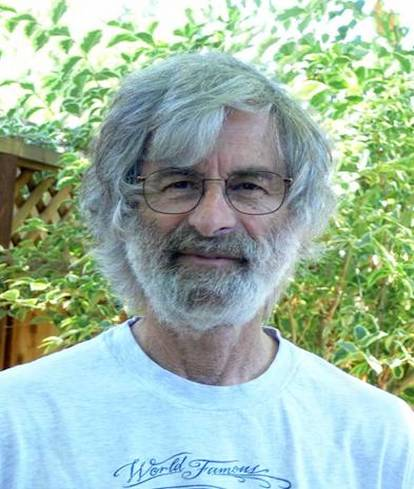
\includegraphics[width=0.47\linewidth]{images/Leslie_Lamport} 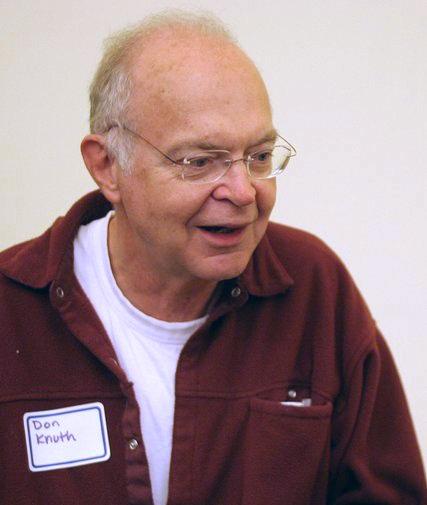
\includegraphics[width=0.47\linewidth]{images/KnuthAtOpenContentAlliance} \caption{\href{https://en.wikipedia.org/wiki/Turing_Award}{Turing award} winners Leslie Lamport and Donald Knuth created TeX and LaTeX during the 1980's. Lamport portrait by Leslie Lamport, GFDL via Wikimedia Commons \href{https://w.wiki/3Daz}{w.wiki/3Daz}, Knuth portrait by Jacob Appelbaum CC BY-SA via Wikimedia Commons \href{https://w.wiki/3Day}{w.wiki/3Day}. Is Donald Knuth the \href{https://www.nytimes.com/2018/12/17/science/donald-knuth-computers-algorithms-programming.html}{The Yoda of Silicon Valley}? \citep{yoda}}\label{fig:knuthport-fig}
\end{figure}



LaTeX is typically used for technical documents but it can be used for almost any form of publishing, including writing CVs, letters, books, posters, presentations and much more. Whatever you create with LaTeX, one of its key strengths is making documents look professional in portable document format (pdf) using industrial-strength typesetting.

\section{LaTeX is NOT a word processor}\label{notword}

By itself, LaTeX is \emph{not} a word processor! Instead, LaTeX encourages you to concentrate on the \emph{content} of your documents, while it takes care of the details of its presentation. This is similar to the approach you've been using for creating web pages in COMP1010 where the style (in your cascading style-sheet: \texttt{*.css}) should be cleanly separated from the raw content (in your \texttt{*.html}). This is a classic abstraction technique in computing by \href{https://en.wikipedia.org/wiki/Separation_of_concerns}{separation of concerns} (SoC). If you're reading this page in a web browser, view the source of this page \texttt{latex.html} as an example, the html only describes the content and says very little about its presentation, that is described separately in the cascading style sheet.

LaTeX is \textbf{not} a what you see is what you get (\href{https://en.wikipedia.org/wiki/WYSIWYG}{WYSIWYG}) system either. The raw document you edit (a \texttt{*.tex} file input) is not your final result (usually a \texttt{*.pdf} file output). LaTeX doesn't even come with a spell-checker, though there are many plug-ins you can use for that, they are not built in.

\section{So what is LaTeX then?}\label{so-what-is-latex-then}

LaTeX is a professional typesetting software system. It can produce documents with a much higher standard of \href{https://en.wikipedia.org/wiki/Typography}{typography} than your average Word processor is capable of. It also has some useful features to help you write scientific and technical documentation, as we will see.

The best way to understand LaTeX is to create some simple documents which we'll do in the next chapter.

\chapter{Simple LaTeX Documents}\label{simples}

Let's start by creating a simple LaTeX document.

\section{A very short document}\label{shortest}

Open up your favourite text editor\footnote{it is worth configuring your editor so that it is LaTeX aware, and can do \href{https://en.wikipedia.org/wiki/Syntax_highlighting}{syntax highlighting}, suggest auto-completions and spell-check for you. Tools like \href{https://code.visualstudio.com/}{VS Code} and \href{https://www.sublimetext.com/}{sublimetext} and many others will do this for you}, enter the following text, then save it as a file called \texttt{turing.tex}:

\begin{Shaded}
\begin{Highlighting}[]
\BuiltInTok{\textbackslash{}documentclass}\NormalTok{[a4paper]\{}\ExtensionTok{article}\NormalTok{\}}
\KeywordTok{\textbackslash{}begin}\NormalTok{\{}\ExtensionTok{document}\NormalTok{\}}
\NormalTok{Computational excursions}
\KeywordTok{\textbackslash{}end}\NormalTok{\{}\ExtensionTok{document}\NormalTok{\}}
\end{Highlighting}
\end{Shaded}

To turn this into a pdf we need to use a LaTeX compiler, we're going to use \texttt{pdflatex}, though several other compilers are available.\footnote{\url{https://www.overleaf.com/learn/latex/Choosing_a_LaTeX_Compiler}} On Linux the \texttt{pdflatex} compiler is already installed and can be used from the command line.\footnote{for example the Linux VM image for VirtualBox \url{https://wiki.cs.manchester.ac.uk/index.php/CSImage_VM}} If you're not using Linux, you'll need to explore the options at \href{https://www.latex-project.org/get/}{latex-project.org/get}.

\begin{Shaded}
\begin{Highlighting}[]
\CommentTok{\# compile turing.tex}
\NormalTok{pdflatex turing.tex}
\CommentTok{\# open the pdf output}
\NormalTok{xdg}\SpecialCharTok{{-}}\NormalTok{open turing.pdf}
\CommentTok{\# or just open turing.pdf on a mac}
\end{Highlighting}
\end{Shaded}

The first command outputs a pdf file from your \texttt{turing.tex} input using the \texttt{pdflatex} compiler. The second command opens the file you've created. If you list the directory contents, you'll see that the compiler has also created an auxillary \texttt{*.aux} file and a \texttt{*.log} file which can be helpful when you're debugging the compilation:

\begin{Shaded}
\begin{Highlighting}[]
\CommentTok{\# files created on compilation}
\NormalTok{turing.tex}
\NormalTok{turing.pdf}
\NormalTok{turing.aux}
\NormalTok{turing.log}
\end{Highlighting}
\end{Shaded}

\section{A longer LaTeX document}\label{longer}

Our \texttt{turing.tex} file is a very simple document, so let's add some sections and fill them out a bit:

\begin{Shaded}
\begin{Highlighting}[]
\BuiltInTok{\textbackslash{}documentclass}\NormalTok{[a4paper]\{}\ExtensionTok{article}\NormalTok{\}}
\KeywordTok{\textbackslash{}begin}\NormalTok{\{}\ExtensionTok{document}\NormalTok{\}}


\KeywordTok{\textbackslash{}section}\NormalTok{\{Algorithms: Cooking Up Programs\}}
\NormalTok{A program specifies in the }\FunctionTok{\textbackslash{}textbf}\NormalTok{\{exact syntax\} of some programming language the computation one expects a computer to perform. The syntax is precise and unforgiving. The slightest error in the program as written may cause the computation to be in error or may halt altogether. The reason for this situation seems paradoxical on the surface: It is relatively easy to design a system that converts rigid syntax to computations; it is much harder to design a system that tolerates mistakes or accepts a broader range of program descriptions.}

\KeywordTok{\textbackslash{}section}\NormalTok{\{Finite automata: The Black Box\}}
\NormalTok{It occasionally happens in industrial, military or educational settings that one is presented with a piece of electronic hardware whose exact function is uncertain or unknown. One way of discovering how the device works is to take it apart, piece by piece, and deduce its function by analysing the components and their interconnections. This is not always possible, however, nor is it always necessary. Given that the mystery machine has both input and output facilities, it may be possible to discover what it does without ever taking it apart. Since its appearance gives no clue about its function, we call it a }\FunctionTok{\textbackslash{}textit}\NormalTok{\{black box\}.}

\KeywordTok{\textbackslash{}section}\NormalTok{\{Systems of Logic: Boolean Bases\}}
\NormalTok{In an age of computers and automation, almost every electronic device one can name incorporates at least one boolean function. For example, many current models of automobile will emit a high{-}pitched whine, buzz or other disturbing noise until their drivers fasten their seat belts. Such a device realises a boolean function of two variables.}

\KeywordTok{\textbackslash{}section}\NormalTok{\{Simulation: The Monte Carlo method\}}
\NormalTok{In the quest to understand the many systems that comprise the modern world we turn increasingly to computer simulation. Whether the system is natural or artificial, frequently one or more of its components have such complex behaviour that the only feasible approach to approximating such behaviour is to assume that it is random.}

\KeywordTok{\textbackslash{}section}\NormalTok{\{Gödel\textquotesingle{}s Theorem: Limits on Logic\}}
\NormalTok{In the early 1930\textquotesingle{}s, Kurt Gödel, a German mathematician, attempted to show that predicate calculus was complete {-} that one can obtain mechanically  (in principle, at least) a proof of any true formula expressed in that calculus. His failure to do this was crowned by the discovery that the task was impossible.}

\KeywordTok{\textbackslash{}section}\NormalTok{\{Can machines think?\}}
\NormalTok{Turing addressed the question \textasciigrave{}\textasciigrave{}Can machines think?\textquotesingle{}\textquotesingle{} in his 1950 paper }\FunctionTok{\textbackslash{}textit}\NormalTok{\{Computing machinery and intelligence\}.}

\KeywordTok{\textbackslash{}section}\NormalTok{\{But what is LaTeX good for?\}}
\NormalTok{We\textquotesingle{}re using this }\FunctionTok{\textbackslash{}LaTeX\textbackslash{} }\NormalTok{document to demonstrate some of its key strengths that you will find useful during and after University:}

\KeywordTok{\textbackslash{}begin}\NormalTok{\{}\ExtensionTok{enumerate}\NormalTok{\}}
\FunctionTok{\textbackslash{}item}\NormalTok{ LaTeX can quickly create pdf files}
\FunctionTok{\textbackslash{}item}\NormalTok{ LaTeX uses professional typesetting}
\FunctionTok{\textbackslash{}item}\NormalTok{ LaTeX documents can be more legible, clear, and visually appealing to the reader than those created with word processing software}
\KeywordTok{\textbackslash{}end}\NormalTok{\{}\ExtensionTok{enumerate}\NormalTok{\}}

\KeywordTok{\textbackslash{}end}\NormalTok{\{}\ExtensionTok{document}\NormalTok{\}}
\end{Highlighting}
\end{Shaded}

The text here is excerpted from \emph{The New Turing Omnibus: 66 excursions in Computer Science} \citep{turingomnibus}. The Omnibus is a lovely introduction to the fundamentals of Computer Science that you might enjoy. In his book review, the software engineer \href{https://en.wikipedia.org/wiki/Jeff_Atwood}{Jeff Atwood} calls the omnibus an ``incredibly fun little book''. \citep{codinghorror}

\section{Exercise one: documentum}\label{ex1}

In your file \texttt{turing.tex} either cut-and-paste this longer text into your document or make your own sections and text. You could use text from \href{https://en.wikipedia.org/wiki/Lorem_ipsum}{Lorem ipsum} at \href{https://www.lipsum.com}{lipsum.com} to fill out the page.

Now, at the top of your document after the \texttt{\textbackslash{}begin\{document\}} line and before first \texttt{\textbackslash{}section}, add the following commands, each on their own line:

\begin{Shaded}
\begin{Highlighting}[]
\FunctionTok{\textbackslash{}title}\NormalTok{\{The New Turing Omnibus\}}
\FunctionTok{\textbackslash{}author}\NormalTok{\{A. K. Dewdney\}}
\FunctionTok{\textbackslash{}maketitle}
\FunctionTok{\textbackslash{}tableofcontents}
\FunctionTok{\textbackslash{}newpage}
\end{Highlighting}
\end{Shaded}

The \texttt{title}, \texttt{author}, \texttt{tableofcontents} and \texttt{newpage} commands are self-explanatory. The \texttt{maketitle} automatically inserts today's date. Your table of contents won't be created until you run pdflatex \textbf{twice} because on the first run, LaTeX gathers and stores information about what to put in the table of contents, and only creates it on the second run.

\begin{Shaded}
\begin{Highlighting}[]
\CommentTok{\# remember to run pdflatex twice for the table of contents}
\NormalTok{pdlfatex turing.tex}
\NormalTok{pdflatex turing.tex}
\end{Highlighting}
\end{Shaded}

\section{Bold, italic and lists}\label{bold-italic-and-lists}

Here's a few points to note about the text above:

\begin{itemize}
\tightlist
\item
  Notice how \textbf{bold} and \emph{italic} formatting are created using \texttt{\textbackslash{}textbf\{\}} and \texttt{\textbackslash{}textit\{\}}
\item
  Notice how lists are created with \texttt{\textbackslash{}item}s inside either \texttt{\textbackslash{}begin\{enumerate\}} for numbered lists or \texttt{\textbackslash{}begin\{itemize\}} for bulleted lists.
\end{itemize}

\section{Quotation marks}\label{quotation-marks}

Typographic or ``curly'' quotation marks are different characters and \emph{not} the same as straight quotes. They look nicer, but you have to remember that unlike straight quotes, open and close quotation marks are different characters:

\begin{itemize}
\tightlist
\item
  open quote \textbf{``} which looks a bit like a miniature \texttt{66}
\item
  close quote \textbf{''} which looks a bit like a miniature \texttt{99}
\end{itemize}

Look carefully at the quotation marks in the text below:

\begin{itemize}
\tightlist
\item
  Turing addressed the question ``Can machines think``\ldots{} ❎
\item
  Turing addressed the question ``Can machines think''\ldots{} ✅
\end{itemize}

In your \texttt{*.tex} file the correct version looks like this

\begin{Shaded}
\begin{Highlighting}[]
\NormalTok{Turing addressed the question \textasciigrave{}\textasciigrave{}Can machines think\textquotesingle{}\textquotesingle{}}
\end{Highlighting}
\end{Shaded}

not

\begin{Shaded}
\begin{Highlighting}[]
\NormalTok{Turing addressed the question \textasciigrave{}\textasciigrave{}Can machines think\textasciigrave{}\textasciigrave{}}
\end{Highlighting}
\end{Shaded}

or

\begin{Shaded}
\begin{Highlighting}[]
\NormalTok{Turing addressed the question \textquotesingle{}\textquotesingle{}Can machines think\textquotesingle{}\textquotesingle{}}
\end{Highlighting}
\end{Shaded}

You've probably never noticed these details because most word processing software\footnote{Microsoft Word, Google Docs etc} tends to auto-correct quotations marks for you. Since LaTeX isn't a word processor (see section \ref{notword}) it leaves your mistakes on the page for all to see. These mistakes are really noticeable in a pdf file and/or printed, so they are worth paying attention to.

\section{Summary}\label{concsimple}

You've created a basic document in LaTeX and we've introduced some of its advantages:

\begin{itemize}
\tightlist
\item
  LaTeX can quickly create pdf files
\item
  LaTeX uses professional typesetting
\item
  LaTeX can create pdf files that look better than those created with conventional word processing software packages
\end{itemize}

Next we'll look at adding some cross-references, figures and citations. This is one thing that LaTeX does much better than your average word processing software which makes it great for editing larger and longer documents, such as your Bachelors, Masters or PhD thesis.

\chapter{Cross-referencing, Illustrating and Citing}\label{figref}

LaTeX has simple but powerful tools to allow you to cross-reference, illustrate and \texttt{cite} sources in your documents, see figure \ref{fig:wikipedian-fig}.

\begin{figure}

{\centering 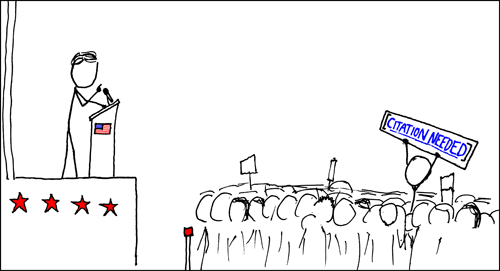
\includegraphics[width=0.7\linewidth]{images/wikipedian_protester} 

}

\caption{It has always been important to cite your sources and LaTeX gives you the tools to cite properly. \emph{Wikipedian Protester} cartoon by \href{https://en.wikipedia.org/wiki/Randall_Munroe}{Randall Munroe} at \href{https://xkcd.com/285/}{xkcd.com/285} published under a \href{https://creativecommons.org/licenses/by-nc/2.5/}{Creative Commons Attribution-NonCommercial 2.5 License}}\label{fig:wikipedian-fig}
\end{figure}



\section{Cross-referencing}\label{cross-referencing}

LaTeX allows you to cross-reference almost anything in your document, including sections, sub-sections, tables and figures. To use the cross-referencing feature you simply insert the command:

\begin{Shaded}
\begin{Highlighting}[]
\KeywordTok{\textbackslash{}label}\NormalTok{\{}\ExtensionTok{mymarker}\NormalTok{\}}
\end{Highlighting}
\end{Shaded}

at the point in the document you want to refer to, and then use the command:

\begin{Shaded}
\begin{Highlighting}[]
\KeywordTok{\textbackslash{}ref}\NormalTok{\{}\ExtensionTok{mymarker}\NormalTok{\}}
\end{Highlighting}
\end{Shaded}

when you want to refer to it. Obviously you replace the text \texttt{mymarker} with something more meaningful. An important tip here is to call the marker something that refers to the content of that part of the document, and to avoid the temptation to use numbers in case you re-order your document. For example, lets say we wanted to cross reference between sections:

\begin{Shaded}
\begin{Highlighting}[]
\BuiltInTok{\textbackslash{}documentclass}\NormalTok{[a4paper]\{}\ExtensionTok{article}\NormalTok{\}}
\KeywordTok{\textbackslash{}begin}\NormalTok{\{}\ExtensionTok{document}\NormalTok{\}}
\KeywordTok{\textbackslash{}section}\NormalTok{\{Turing Machines: The Simplest Computers\}}
\KeywordTok{\textbackslash{}label}\NormalTok{\{}\ExtensionTok{sec:simplest}\NormalTok{\}}
\NormalTok{Turing machines are the simplest and most widely used theoretical models of computing. Far too slow and unwieldy ever to be embodied in a real device, these conceptual machines nevertheless seem to capture everything we mean by the term }\FunctionTok{\textbackslash{}textit}\NormalTok{\{computation\}. Not only do Turing machines occupy the top level of the Chomsky hierarchy, but they also seem capable of computing any function which is computable by any other conceptual scheme.}

\KeywordTok{\textbackslash{}section}\NormalTok{\{Alan Turing\}}
\NormalTok{The Turing machines described in section }\KeywordTok{\textbackslash{}ref}\NormalTok{\{}\ExtensionTok{sec:simplest}\NormalTok{\} are named after Alan Turing.}
\KeywordTok{\textbackslash{}end}\NormalTok{\{}\ExtensionTok{document}\NormalTok{\}}
\end{Highlighting}
\end{Shaded}

\section{Illustrating your documents}\label{illustrating-your-documents}

Documents without figures, images, pictures and graphs are pretty dull, so you'll want to illustrate your document with figures such as the one in Figure \ref{fig:turing-fig}, for example.

\begin{figure}

{\centering 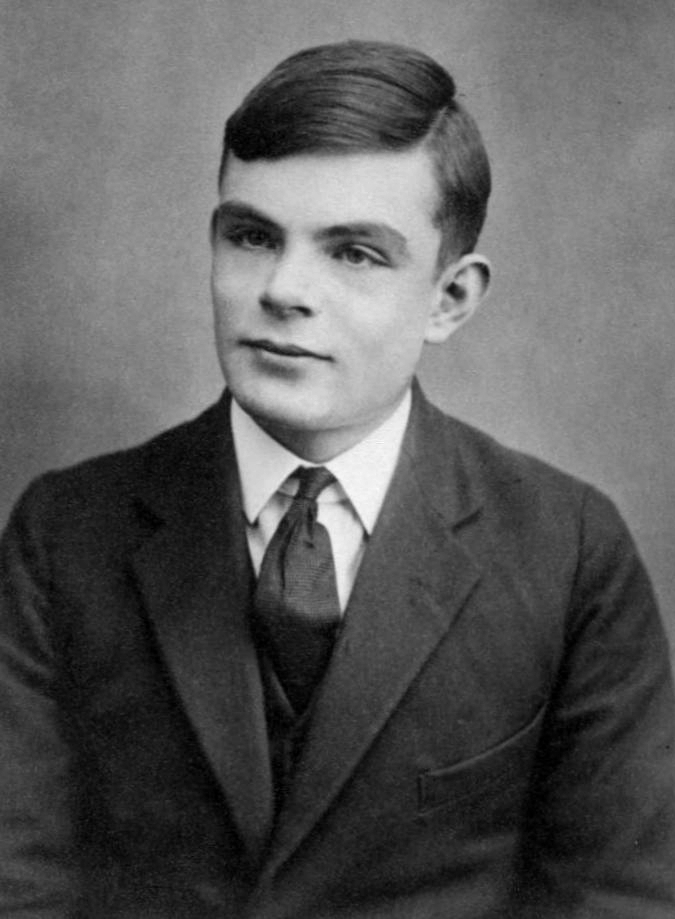
\includegraphics[width=0.4\linewidth]{images/Alan_Turing_Aged_16} 

}

\caption{\href{https://en.wikipedia.org/wiki/Alan_Turing}{Alan Turing} at the age of sixteen, portrait by unknown author, public domain, via Wikimedia Commons \href{https://w.wiki/oZx}{w.wiki/oZx}}\label{fig:turing-fig}
\end{figure}



Including figures and pictures in your document is straightforward. You do it like this:

\begin{Shaded}
\begin{Highlighting}[]
\KeywordTok{\textbackslash{}begin}\NormalTok{\{}\ExtensionTok{figure}\NormalTok{\}}
\BuiltInTok{\textbackslash{}includegraphics}\NormalTok{[width=10cm]\{}\ExtensionTok{images/turing.jpg}\NormalTok{\}}
\FunctionTok{\textbackslash{}caption}\NormalTok{\{Turing machines are named after Alan Turing\}}
\KeywordTok{\textbackslash{}label}\NormalTok{\{}\ExtensionTok{figure:turing}\NormalTok{\}}
\KeywordTok{\textbackslash{}end}\NormalTok{\{}\ExtensionTok{figure}\NormalTok{\}}
\end{Highlighting}
\end{Shaded}

The command \texttt{\textbackslash{}includegraphics\{\}} gets your image, which can be PDF, PNG, JPG, GIF or PostScript. The \texttt{\textbackslash{}begin\{figure\}} and \texttt{\textbackslash{}end\{figure\}} code wraps up whatever picture you're including, and allows LaTeX to treat it as an unbreakable floating thing that it will position for you as best it can in the document, while maintaining an overall nice typographical layout. This ``floating'' of figures can sometimes result in the figure ending up in a place you didn't expect, but in most cases LaTeX will make the most sensible choice. It's possible to employ finer control over figure placement, but that's beyond the scope of this guide.

The \texttt{\textbackslash{}includegraphics} command is not built in to core LaTeX but is in an additional package, which needs to be explicitly loaded. You can load this package by using the command \texttt{usepackage} in the document preamble, in between the \texttt{\textbackslash{}documentclass} and the \texttt{\textbackslash{}begin\{document\}}.

\begin{Shaded}
\begin{Highlighting}[]
\BuiltInTok{\textbackslash{}documentclass}\NormalTok{[a4paper]\{}\ExtensionTok{article}\NormalTok{\}}
\BuiltInTok{\textbackslash{}usepackage}\NormalTok{\{}\ExtensionTok{graphicx}\NormalTok{\}}
\KeywordTok{\textbackslash{}begin}\NormalTok{\{}\ExtensionTok{document}\NormalTok{\}}
\end{Highlighting}
\end{Shaded}

\section{Exercise two: picture this}\label{ex2}

Create a document \texttt{image.tex}, that contains some text (maybe from Lorem Ipsum), together with a figure containing an image of your choice. Create a cross reference to the figure in the text.

\section{Citations and footnotes}\label{citations-and-footnotes}

Footnotes\footnote{This is a footnote about footnotes. Very meta.} can be added to a document with \texttt{\textbackslash{}footnote\{\}}

\begin{Shaded}
\begin{Highlighting}[]
\FunctionTok{\textbackslash{}footnote}\NormalTok{\{This is a footnote about footnotes\}}
\end{Highlighting}
\end{Shaded}

You can cite sources such as websites, books or journal articles in your document using the \texttt{\textbackslash{}cite} command.

\begin{Shaded}
\begin{Highlighting}[]
\KeywordTok{\textbackslash{}cite}\NormalTok{\{}\ExtensionTok{alanturing}\NormalTok{\}}
\end{Highlighting}
\end{Shaded}

The metadata for the citations can be stored in a separate \texttt{*.bib\ file} using a format called BibTeX, in this case we'll use \texttt{turing.bib}. BibTeX provides citation types so books are described using the \texttt{@book} type like this:

\begin{Shaded}
\begin{Highlighting}[]
\NormalTok{@Book\{turingomnibus,}
\NormalTok{  title = \{The New Turing Omnibus: Sixty{-}six excursions in Computer Science\},}
\NormalTok{  author = \{A. K. Dewdney\},}
\NormalTok{  publisher = \{Henry Holt\},}
\NormalTok{  address = \{New York\},}
\NormalTok{  year = \{2001\},}
\NormalTok{  isbn = \{9780805071665\},}
\NormalTok{  url = \{https://en.wikipedia.org/wiki/Special:BookSources?isbn=978{-}0805071665\}}
\NormalTok{\}}
\end{Highlighting}
\end{Shaded}

and articles\footnote{BibTeX entries for journal articles can be automatically generated from persistent identifiers known as \href{https://en.wikipedia.org/wiki/Digital_object_identifier}{digital object identifiers} or doi's, such as \url{https://doi2bib.org} for example. This saves you the unpleasant, time consuming and error prone task of typing them in by hand.} use the \texttt{@article} type like this:

\begin{Shaded}
\begin{Highlighting}[]
\NormalTok{@article\{alanturing,}
\NormalTok{  doi = \{10.1112/plms/s2{-}42.1.230\},}
\NormalTok{  url = \{https://doi.org/10.1112/plms/s2{-}42.1.230\},}
\NormalTok{  year = \{1937\},}
\NormalTok{  publisher = \{Wiley\},}
\NormalTok{  volume = \{s2{-}42\},}
\NormalTok{  number = \{1\},}
\NormalTok{  pages = \{230{-}{-}265\},}
\NormalTok{  author = \{Alan Turing\},}
\NormalTok{  title = \{On Computable Numbers, with an Application to the Entscheidungsproblem\},}
\NormalTok{  journal = \{Proceedings of the London Mathematical Society\}}
\NormalTok{\}}
\end{Highlighting}
\end{Shaded}

For everything else\footnote{There are many other types of BibTeX entries besides articles, books and misc. See \url{https://en.wikibooks.org/wiki/LaTeX/Bibliography_Management\#BibTeX}} you can use the \texttt{@misc} type:

\begin{Shaded}
\begin{Highlighting}[]
\NormalTok{@misc\{googlescholar,}
\NormalTok{  author       = \{Anon\},}
\NormalTok{  title        = \{Alan Turing Google Scholar page\},}
\NormalTok{  url          = \{https://scholar.google.co.uk/citations?user=VWCHlwkAAAAJ\},}
\NormalTok{  year         = \{2022\},}
\NormalTok{\}}
\end{Highlighting}
\end{Shaded}

So to create the text:

``\emph{You can find Turing's publications in Google scholar. \citep{googlescholar}
His paper on the Entscheidungsproblem was published in 1937. \citep{turing}
He wrote about thinking machines in 1950. \citep{turing50}}''

You add this to your tex file:

\begin{Shaded}
\begin{Highlighting}[]
\NormalTok{You can find Turing\textquotesingle{}s publications in Google scholar. }\KeywordTok{\textbackslash{}cite}\NormalTok{\{}\ExtensionTok{googlescholar}\NormalTok{\}}
\NormalTok{His paper on the Entscheidungsproblem was published in 1937. }\KeywordTok{\textbackslash{}cite}\NormalTok{\{}\ExtensionTok{alanturing}\NormalTok{\}}
\NormalTok{He wrote about thinking machines in 1950. }\KeywordTok{\textbackslash{}cite}\NormalTok{\{}\ExtensionTok{turing50}\NormalTok{\}}
\end{Highlighting}
\end{Shaded}

To generate your bibliography you'll need to specify what style of bibliography you're using with \texttt{\textbackslash{}bibliographystyle\{stylename\}} and where to find the metadata with \texttt{\textbackslash{}bibliography\{bibfile\}}. The example below uses a style called \texttt{unsrt} and uses a bib file called \texttt{turing.bib} which might contain many articles and books. You don't need to specific the file extension \texttt{.bib}:

\begin{Shaded}
\begin{Highlighting}[]
\BuiltInTok{\textbackslash{}bibliographystyle}\NormalTok{\{}\ExtensionTok{unsrt}\NormalTok{\}}
\BuiltInTok{\textbackslash{}bibliography}\NormalTok{\{}\ExtensionTok{turing}\NormalTok{\}}
\end{Highlighting}
\end{Shaded}

When you compile you need to run \texttt{pdflatex} before and after running \texttt{bibtex} like this:

\begin{Shaded}
\begin{Highlighting}[]
\NormalTok{pdflatex turing.tex}
\NormalTok{bibtex turing}
\NormalTok{pdflatex turing.tex}
\NormalTok{pdflatex turing.tex}
\end{Highlighting}
\end{Shaded}

If you find all the typing at the command line tedious, you could write a little bash script to automate this simple workflow including opening the pdf when it is created.

\section{Summary}\label{fingconc}

You have cross-referenced, illustrated, added citations and footnotes to your document. Next we'll look at doing some maths.

\chapter{Doing the Maths}\label{maths}

LaTeX provides powerful tools for typesetting mathematics and this chapter looks at some of them.

If you can't see the equations and matrix below in your web browser, you'll need to use the pdf or epub version of this manual at \href{https://latex4year1.netlify.app/latex4year1.pdf}{latex4year1.pdf} or \href{https://latex4year1.netlify.app/latex4year1.epub}{latex4year1.epub}. Otherwise, if you can see the equation below, it is safe to read on\ldots{}

\section{Equations}\label{equations}

Consider this equation:

\[ x = \frac{-b \pm \sqrt{b^2-4ac}}{2a} \]

To render the equation, you include this in your tex file:

\begin{Shaded}
\begin{Highlighting}[]
     \SpecialStringTok{\textbackslash{}[ x = }\SpecialCharTok{\textbackslash{}frac}\SpecialStringTok{\{{-}b }\SpecialCharTok{\textbackslash{}pm}\SpecialStringTok{ }\SpecialCharTok{\textbackslash{}sqrt}\SpecialStringTok{\{b\^{}2{-}4ac\}\}\{2a\} \textbackslash{}]}
\end{Highlighting}
\end{Shaded}

You can probably work out how most of this creates the formula, but it won't be obvious that the \texttt{\textbackslash{}{[}} and \texttt{\textbackslash{}{]}} symbols that enclose the formula mean typeset this as a displayed formula, giving it some vertical space from the surrounding text. If we'd used \texttt{\textbackslash{}(} and \texttt{\textbackslash{})} instead to enclose the formula it would appear in-line, like this: \(x = \frac{-b \pm \sqrt{b^2-4ac}}{2a}\). It still looks very nice, and observe how it's automatically been resized to fit, and that the lines of text have had their spacing changed a bit. This all looks simple, but the implementation inside LaTeX and TeX is complex. It involves parsing the description of the formula to create a corresponding tree data structure, which is then recursively walked to work out the horizontal and vertical typographical spacings needed. You'll meet these ideas in COMP11120 Mathematical Techniques for Computer Science in your first year and COMP26120 Algorithms in your second year.

Here's another example, taken from computer graphics, it's a local illumination model incorporating ambient, diffuse and specular reflection by multiple lights:

\[ I = k_a I_a + \sum_{i=1}^M {\frac{{I_p}_i}{d'_i}} [ k_d(\hat{N}\cdot\hat{L_i}) + k_s(\hat{R_i}\cdot\hat{V})^n] \]

We write this in LaTeX as follows:

\begin{Shaded}
\begin{Highlighting}[]
    \SpecialStringTok{\textbackslash{}[ I = k\_a I\_a + }\SpecialCharTok{\textbackslash{}sum}\SpecialStringTok{\_\{i=1\}\^{}M \{ }\SpecialCharTok{\textbackslash{}frac}\SpecialStringTok{\{\{I\_p\}\_i\}\{d\textquotesingle{}\_i\} \}}
\SpecialStringTok{    [ k\_d(}\SpecialCharTok{\textbackslash{}hat}\SpecialStringTok{\{N\} }\SpecialCharTok{\textbackslash{}cdot}\SpecialStringTok{ }\SpecialCharTok{\textbackslash{}hat}\SpecialStringTok{\{L\_i\})}
\SpecialStringTok{    + k\_s(}\SpecialCharTok{\textbackslash{}hat}\SpecialStringTok{\{R\_i\} }\SpecialCharTok{\textbackslash{}cdot}\SpecialStringTok{ }\SpecialCharTok{\textbackslash{}hat}\SpecialStringTok{\{V\})\^{}n] \textbackslash{}]}
\end{Highlighting}
\end{Shaded}

Try to match the LaTeX commands with the formula displayed above. You'll see lots of curly brackets, and this example illustrates their two uses in LaTeX. The first is to provide an argument to a command; for example \texttt{\textbackslash{}hat\{N\}} means apply the \texttt{\textbackslash{}hat} command to \(N\)', which creates \(\hat{N}\), the vector \(N\) with a little hat on.

The second use of curly brackets is to group things together to avoid ambiguities. In the example you can see \(\sum_{i=1}^M\), which creates a summation sign and its lower and upper limits: \(\sum_{i=1}^{M}\). We wrap the lower bound, \texttt{i=1} in curly brackets to group it into an indivisible unit. If we were to omit the brackets, writing \texttt{\textbackslash{}sum\_i=1\^{}M}, LaTeX would then produce \(\sum_i=1^M\), which is not at all what we want (even LaTeX can't always know what we really want).

\section{Matrices}\label{matrix}

As well as equations, LaTeX can display matrices. This one expresses a particular 3D geometrical transformation:

\[ T_1 = \left[
 \begin{array}{cccc}
 \cos \theta & -\sin \theta & 0 & \delta \\
 \sin \theta  & \cos \theta & 0 & \epsilon \\
 0 & 0 & 1 & \eta \\
 \alpha & \beta & \gamma & 1
 \end{array}
 \right] \]

The source for this matrix looks like this:

\begin{Shaded}
\begin{Highlighting}[]
   \SpecialStringTok{\textbackslash{}[ T\_1 = }\SpecialCharTok{\textbackslash{}left}\SpecialStringTok{[}
\SpecialStringTok{    }\KeywordTok{\textbackslash{}begin}\NormalTok{\{}\ExtensionTok{array}\NormalTok{\}}\SpecialStringTok{\{cccc\}}
\SpecialStringTok{    }\SpecialCharTok{\textbackslash{}cos}\SpecialStringTok{ }\SpecialCharTok{\textbackslash{}theta}\SpecialStringTok{ \& {-}}\SpecialCharTok{\textbackslash{}sin}\SpecialStringTok{ }\SpecialCharTok{\textbackslash{}theta}\SpecialStringTok{ \& 0 \& }\SpecialCharTok{\textbackslash{}delta}\SpecialStringTok{ }\SpecialCharTok{\textbackslash{}\textbackslash{}}
\SpecialStringTok{    }\SpecialCharTok{\textbackslash{}sin}\SpecialStringTok{ }\SpecialCharTok{\textbackslash{}theta}\SpecialStringTok{  \& }\SpecialCharTok{\textbackslash{}cos}\SpecialStringTok{ }\SpecialCharTok{\textbackslash{}theta}\SpecialStringTok{ \& 0 \& }\SpecialCharTok{\textbackslash{}epsilon}\SpecialStringTok{ }\SpecialCharTok{\textbackslash{}\textbackslash{}}
\SpecialStringTok{    0 \& 0 \& 1 \& }\SpecialCharTok{\textbackslash{}eta}\SpecialStringTok{ }\SpecialCharTok{\textbackslash{}\textbackslash{}}
\SpecialStringTok{    }\SpecialCharTok{\textbackslash{}alpha}\SpecialStringTok{ \& }\SpecialCharTok{\textbackslash{}beta}\SpecialStringTok{ \& }\SpecialCharTok{\textbackslash{}gamma}\SpecialStringTok{ \& 1}
\SpecialStringTok{    }\KeywordTok{\textbackslash{}end}\NormalTok{\{}\ExtensionTok{array}\NormalTok{\}}
\SpecialStringTok{    }\SpecialCharTok{\textbackslash{}right}\SpecialStringTok{] \textbackslash{}]}
\end{Highlighting}
\end{Shaded}

In the LaTeX code, \texttt{\textbackslash{}left{[}} means `big opening square bracket please'; \texttt{\{cccc\}} means `an array with 4 columns please, with the items in each column centred'; \texttt{\&} means `start a new column'; and \texttt{\textbackslash{}\textbackslash{}} means `start a new row'. You'll notice that LaTeX knows about greek letters; it knows about most standard maths symbols too, and also the ways they're usually used.

There are some symbols that you might need (for example \texttt{\textbackslash{}therefore}, which produces the usual three dots symbol ∴) that are not part of standard LaTeX. Many such symbols are provided by the \texttt{amssymb} package of symbols compiled by the American Mathematical Society. Details of the many symbols provided by this package can be found online. To use these extra symbols, you need to have \texttt{\textbackslash{}usepackage\{amssymb\}} in your document preamble.

LaTeX really shines at typesetting mathematics, we've really only scratched the surface here. For more have a look at
\href{https://en.wikibooks.org/wiki/LaTeX/Mathematics}{en.wikibooks.org/wiki/LaTeX/Mathematics} or books such as the \emph{Guide to LaTeX} by Helmut Kopka and Patrick W. Daly. \citep{kopka}

\section{Exercise three: you do the maths}\label{ex3}

Now for an exercise that involves some mathematics. Create a file \texttt{maths.tex} which typesets the following piece of text and mathematics:

There are many positive integer solutions to the equation

\[ x^2 + y^2 =  z^2 \]

which can be rewritten as

\[ z = \sqrt{x^2 + y^2} \]

For example \((3,4, 5)\) or \((5,12,13)\). Such solutions are called \emph{Pythagorean triples}.

However, for higher powers the situation is very different, and we have:-

\textbf{Theorem: Fermat-Wiles}
For all natural numbers \(n ≥ 3\), there are no integers \(x,y,z\) satisfying the equation:

\[ x^n + y^n = z^n \]

\section{Summary}\label{mathconc}

We've briefly introduced typesetting mathematics in LaTeX with some equations and a matrix. LaTeX can handle a lot more maths than that but this gives you a flavour of what it can do. In the next chapter we'll look at collaborative authoring and editing in the cloud with overleaf.

\chapter{Collaborative Editing in the Cloud with Overleaf}\label{overleaf}

If you are the sole author of a document, then compiling files on your local machine is fine. However, if you need to collaboratively co-author a document with other people, you'll need to share your TeX somehow. Sharing \texttt{*.tex} files by email or dropbox or whatever would be cumbersome. What you need is something like Google Docs for \texttt{*.tex}. Overleaf (\href{https://www.overleaf.com/}{overleaf.com}) is one of several web applications that allows you to do this, shown in the screenshot in Figure \ref{fig:overleaf-fig}.

\begin{figure}

{\centering 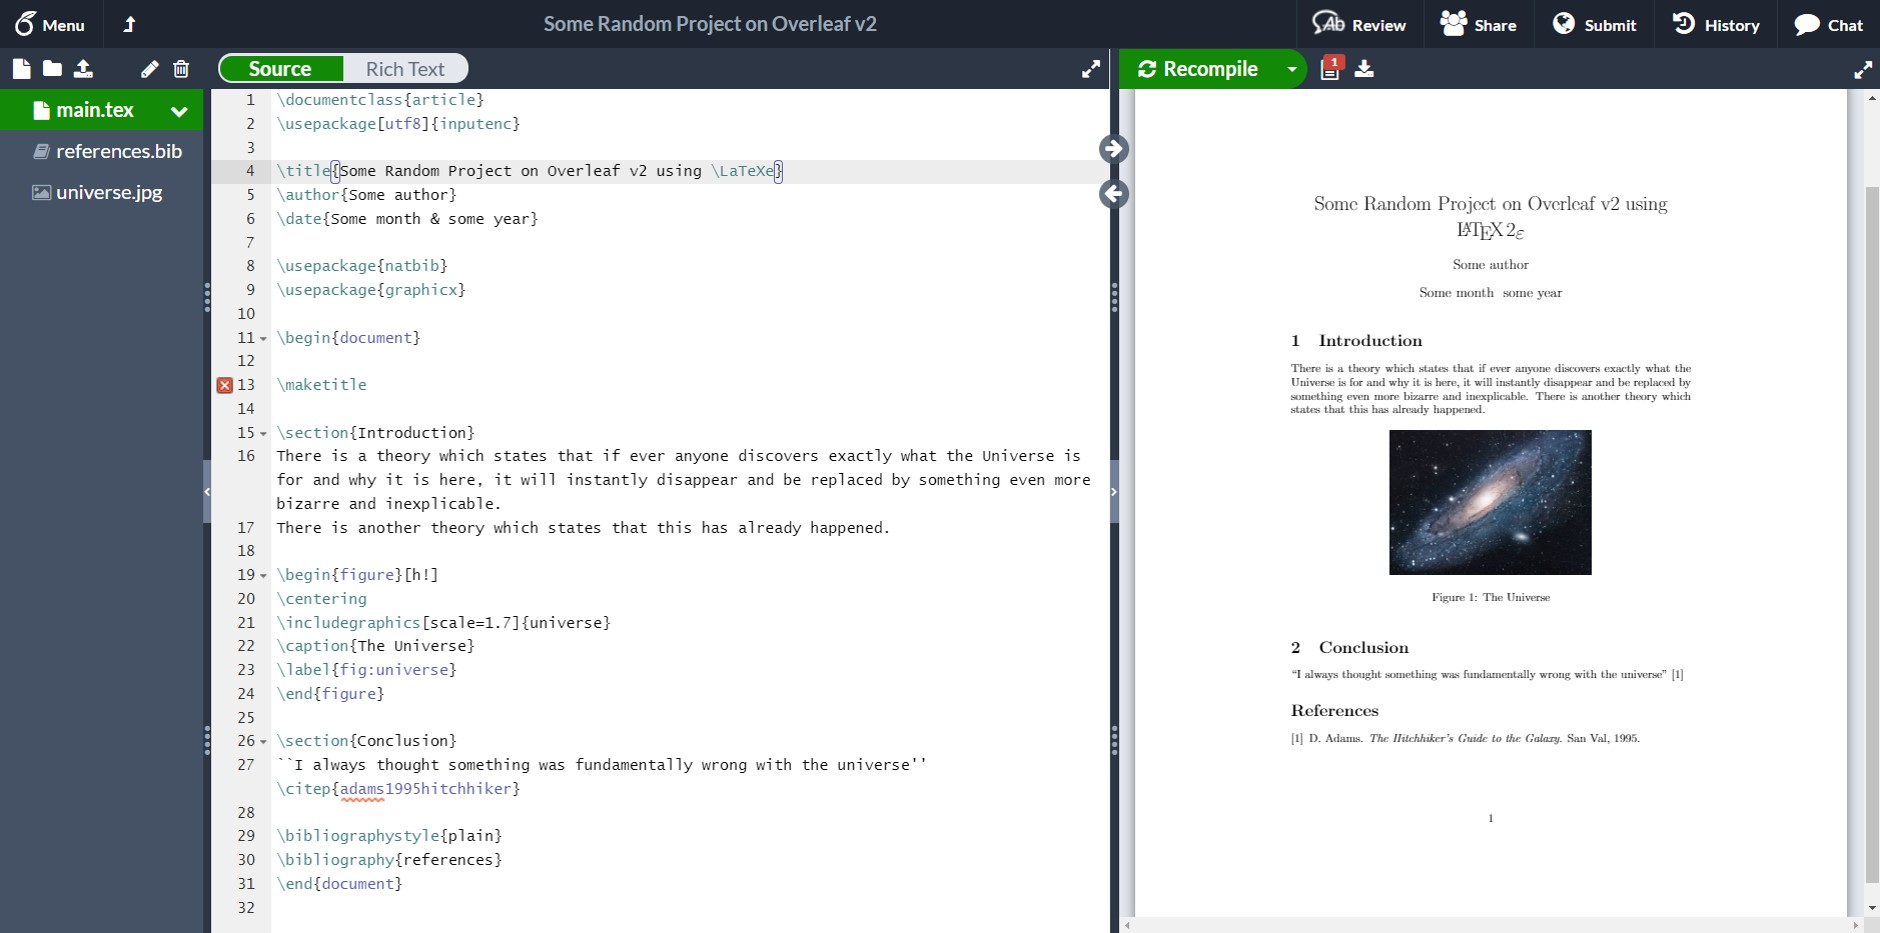
\includegraphics[width=1\linewidth]{images/Overleaf_v2_editing_page} 

}

\caption{A screenshot of overleaf showing the source TeX on the left hand side and the corresponding pdf on the right hand side. Screenshot by Dan Cherniy via Wikimedia Commons at \href{https://w.wiki/omo}{w.wiki/omo}}\label{fig:overleaf-fig}
\end{figure}



Compared to LaTeX, overleaf is relatively new. Write Latex Limited, the company behind overleaf was founded fairly recently (in LaTeX terms) in 2013 by \href{https://www.linkedin.com/in/jdleesmiller/}{John Lees-Miller} and \href{https://www.linkedin.com/in/john-hammersley-6419a266/}{John Hammersley}. Overleaf has several features which you might find useful:

\begin{itemize}
\tightlist
\item
  Your documents are automatically saved to the cloud
\item
  Packages, class files, compilers and other LaTeX components are also in the cloud, saving you time installing and managing them
\item
  Templates are provided for common types of documents, although you don't need to use overleaf to get access to LaTeX templates\footnote{see \url{http://www.tug.org/texshowcase} and \url{https://www.latextemplates.com} for example}
\item
  Overleaf publish lots of tutorials to help you learn LaTeX
\end{itemize}

\section{Exercise four: overleaf}\label{ex4}

Login to \href{https://www.overleaf.com/}{overleaf.com} and try the following:

\begin{enumerate}
\def\labelenumi{\arabic{enumi}.}
\tightlist
\item
  Create and save a simple document using the overleaf tutorial \emph{creating a document in overleaf}\footnote{\url{https://www.overleaf.com/learn/how-to/Creating_a_document_in_Overleaf}}\strut \\
\item
  Note that overleaf allows you to store your TeX source in a git repository so you can use version control if you want to
\item
  Browse the overleaf tutorials at \href{https://www.overleaf.com/learn}{overleaf.com/learn} and ask questions on forums like \href{https://tex.stackexchange.com/}{tex.stackexchange.com} if you want to take things further
\end{enumerate}

\section{Summary}\label{overleafconc}

Overleaf provides a modern and convenient cloud based interface to tried and tested LaTeX tools, which have been around for over thirty years. \citep{knuth} It also allows you to share the source of your documents while providing some handy templates for common document types. Overleaf and the command line are just two popular interfaces to LaTeX amongst many others. \citep{latexproject} Which interface is ``best'' for you will largely depend on what kind of documents you are writing and what your workflow is. In the next chapter we will create a curriculum vitae using CV templates provided by overleaf.

\chapter{Your Curriculum Vitae}\label{cv}

You'll write many documents at University, but there is one document that is \textbf{really} important in a potentially life-changing way. Your curriculum vitae\footnote{strictly speaking it should be vitæ (not vitae) if you're being pedantic} or resume. An example CV is shown in Figure \ref{fig:cv-fig}.

\begin{figure}

{\centering 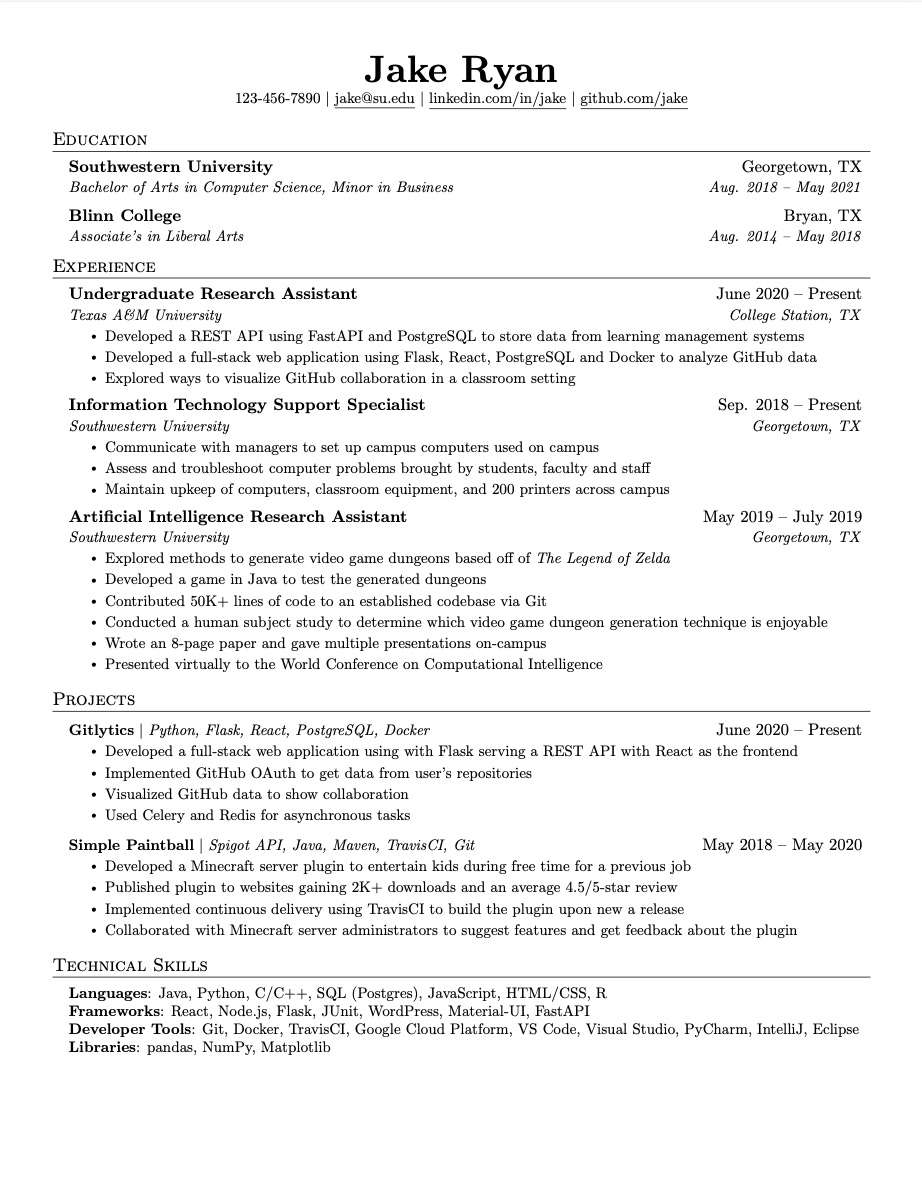
\includegraphics[width=1\linewidth]{images/jake-ryan} 

}

\caption{A fictitious example CV using an overleaf template. Would you invite Neil to interview based on his CV? This is what your CV needs to do, convince a decision maker they really need to contact you to find out more. This is just a screenshot, the pdf can be found at \href{https://www.cdyf.me/Neil_Pointer.pdf}{cdyf.me/Neil\_Pointer.pdf}. There are over 600 CV templates available to choose from at \href{https://www.overleaf.com/gallery/tagged/cv}{overleaf.com/gallery/tagged/cv} for you to choose from.}\label{fig:cv-fig}
\end{figure}



Creating a professional looking CV is particularly important, because it determines if you are invited to interview for \emph{opportunities} you are applying for. The decision to interview is typically based on several factors:

\begin{itemize}
\tightlist
\item
  how your CV looks, the typesetting and style (typography)
\item
  the content of your CV, what you've done
\item
  the quality and clarity of your written communication, how you describe yourself and your experience
\item
  the editing, what you've decided to leave in (and leave out) of your CV
\end{itemize}

\section{Using your CV to get a job interview}\label{knocking}

By \emph{opportunities} we mean both immediate ones within the next 12 months as well as those further in the future. To make the most of those opportunities, your CV needs to be persuasive enough to make an employer think they should invite you to interview.

\subsection{Job opportunities for first year students}\label{startearly}

During your first year of study, \emph{opportunities} include insight events and summer internships:

\begin{itemize}
\tightlist
\item
  Spring insights, usually occur during easter vacation, and require you to apply before (or shortly after) Christmas, see

  \begin{itemize}
  \tightlist
  \item
    insight events at \href{https://bit.ly/gradcracker-spring-insights}{bit.ly/gradcracker-spring-insights}
  \item
    and \href{https://www.ratemyplacement.co.uk/insights}{ratemyplacement.co.uk/insights}
  \end{itemize}
\item
  Summer internships suitable for first year, see:

  \begin{itemize}
  \tightlist
  \item
    summer internships (open to first years) at \href{https://bit.ly/gradcracker-first-years}{bit.ly/gradcracker-first-years}
  \item
    the chapter on \emph{\href{https://www.cdyf.me/finding}{Finding your Future}} in \emph{Coding your Future} \citep{findingyourfuture} for other places you can look
  \end{itemize}
\end{itemize}

\subsection{Subsequent opportunities}\label{afterfirst}

After your first year \emph{opportunities} include:

\begin{itemize}
\tightlist
\item
  Year long placements in your penultimate year, if you're considering doing \href{http://studentnet.cs.manchester.ac.uk/employment/placement/}{industrial experience}
\item
  Summer internships (aimed at penultimate year students)
  + there are usually around ten summer internships in the Department of Computer Science for example, these \emph{normally} don't get advertised around April/May time
\item
  Graduate jobs or graduate schemes after graduation
\item
  Postgraduate study or research via masters or PhD etc
\end{itemize}

Any time you invest in creating a convincing CV will pay off in the long run. Yes, you've only just started University, so might not have much to talk about just yet, but it's never too early to make a start.

\section{Exercise five: your CV}\label{ex5}

Create a basic CV which tells your story, in particular:

\begin{itemize}
\tightlist
\item
  your \emph{education}, including high school and University
\item
  your \emph{experience}, voluntary, paid, casual, technical and non-technical: \emph{any} experience demonstrates your range of soft and hard skills
\item
  your \emph{projects}, personal, social, educational and entrepreneurial
\end{itemize}

You can do this using the ready-made templates at \href{https://www.overleaf.com/gallery/tagged/cv}{overleaf.com/gallery/tagged/cv}. Have a good look around, there are over 600 templates to choose from.

\section{Beware of weird LaTeX templates}\label{weird}

LaTeX packages like \href{https://www.overleaf.com/learn/latex/Hyperlinks}{hyperref} are used in several of the CV templates above. They sometimes default to weird and unusual styles, such as drawing an ugly cyan box around hyperlinks using \texttt{urlcolor-cyan}. This looks horrible, but you can over-ride by using something like this:

\begin{Shaded}
\begin{Highlighting}[]
\FunctionTok{\textbackslash{}href}\NormalTok{\{https://www.cdyf.me\}\{}\FunctionTok{\textbackslash{}textcolor}\NormalTok{\{blue\}\{}\FunctionTok{\textbackslash{}underline}\NormalTok{\{cdyf.me\}\}\}}
\end{Highlighting}
\end{Shaded}

\section{Debugging your CV checklist}\label{debugging-your-cv-checklist}

As you progress through University, continuously update your CV and solicit feedback from as many people as you can. Your fellow students, personal tutors, friends, family and anyone else you trust can all give you valuable feedback. There will be opportunities to debug your CV later, but you'll need a ``beta release'' (version 1.0) of your CV to get started. The best time to start debugging is now, so that you can squash any bugs before employers see them. Innocent bugs \textbf{can be fatal} because most employers typically have to deal with lots of applicants. Here's a check list of some common bugs we have seen in students CVs:

\begin{enumerate}
\def\labelenumi{\arabic{enumi}.}
\tightlist
\item
  Is your year of graduation, degree program, University and expected (or achieved) degree classification clear?
\item
  Are there any spelling mistakes, typos and grammatical errors? Don't just rely on a spellchecker, they can't detect everything
\item
  Does it look good, decent layout, easy to scan?
\item
  Does it fit comfortably on one page (preferably) or two pages only? Not too cramped or gappy?
\item
  Is it in reverse chronological order? Are the most important (usually recent) things first?
\item
  Have you talked about what you have actually done using prominent verbs, rather than just what you know? See the \emph{\href{https://www.cdyf.me/verbalising}{Verbalising your Future}} chapter of \emph{Coding your Future} for more examples
\item
  Have you mentioned disciplines you are studying now and throughout the current academic year, not just courses you have finished?
\item
  Have you quantified and provided evidence for the claims you make?
\item
  Is your CV robot proof? Many large employers use automated applicant tracking systems that use software to screen CVs long before a human ever sees them. You can feed your CV through software like \href{http://careerset.com/manchester}{careerset.com/manchester} and \href{https://resume.io/}{resume.io}, what feedback do the robots give you? How can you make your CV more robot proof?
\item
  Find out more in the \emph{debugging your future} checklist at \href{https://www.cdyf.me/debugging\#checklist}{cdyf.me/debugging\#checklist} \citep{debugyourfuture}
\item
  If you're a University of Manchester student, take a look at the CV pathway from the careers service at \href{https://bit.ly/uomcvpathway}{bit.ly/uomcvpathway} which requires a \texttt{careerconnect.manchester.ac.uk} login - unfortunately \emph{not} the same as your University credentials
\end{enumerate}

\section{Summary}\label{cvconc}

Your curriculum vitae is a \emph{really} important document and it will most likely take many iterations to get it right. We recommend you start working on it sooner rather than later and get feedback from as many different people (and bots) as you reasonably can.

In the meantime, enjoy exploring and using LaTeX to create professional documents for:

\begin{itemize}
\tightlist
\item
  your individual COMP101 coursework (see blackboard)
\item
  your CV / resume
\item
  your third year project dissertation. It might seem a long way off now but it comes around very quickly!
\end{itemize}

\ldots and more.

\appendix


\chapter{Typography}\label{typography}

A mostly empty placeholder appendix which will cover some typographical details about \href{https://en.wikipedia.org/wiki/Kerning}{kerning} and \href{https://en.wikipedia.org/wiki/Orthographic_ligature}{ligatures} etc.

  \bibliography{book.bib}

\end{document}
